	\documentclass[a4paper,12pt]{report}
\usepackage[utf8]{vietnam}
\usepackage{amsmath}
\usepackage{amsfonts}
\usepackage{enumitem}
%\usepackage{amssymb}
\usepackage{graphicx}
%\usepackage{cases}
\usepackage{fancybox}
\usepackage{multirow}
\usepackage{longtable}
\usepackage{listings}
\usepackage[nottoc]{tocbibind}
\usepackage{indentfirst}
\usepackage[english]{babel}
\usepackage{float}
\PassOptionsToPackage{hyphens}{url}\usepackage{hyperref}  
\usepackage[left=3cm, right=2.00cm, top=2.00cm, bottom=2.00cm]{geometry}
%\lstset{
   %keywords={break,case,catch,continue,else,elseif,end,for,function,
   %   global,if,otherwise,persistent,return,switch,try,while},
%   language = Java,
%   basicstyle=\ttfamily \fontsize{12}{15}\selectfont,   
	% numbers=left,
%   frame=lrtb,
%tabsize=3
%}
\hypersetup{
    colorlinks,
    citecolor=black,
    filecolor=black,
    linkcolor=blue,
    urlcolor=red 
}
\setlength{\parskip}{0.6em}
\addto\captionsenglish{%
 \renewcommand\chaptername{Phần}
 \renewcommand{\contentsname}{Mục lục} 
 \renewcommand{\listtablename}{Danh sách bảng}
 \renewcommand{\listfigurename}{Danh sách hình vẽ}
 \renewcommand{\tablename}{Bảng}
 \renewcommand{\figurename}{Hình}
 \renewcommand{\bibname}{Tài liệu tham khảo}
}

%\newtheorem{definition}{Định nghĩa}[chapter]
%\newtheorem{lema}{Bổ đề}[chapter]
%\newtheorem{theorem}{Định lý}[chapter]

\begin{document}
\thispagestyle{empty}
\thisfancypage{
\setlength{\fboxrule}{1pt}
\doublebox}{}

\begin{center}
{\fontsize{16}{19}\fontfamily{cmr}\selectfont TRƯỜNG ĐẠI HỌC BÁCH KHOA HÀ NỘI\\
VIỆN CÔNG NGHỆ THÔNG TIN VÀ TRUYỀN THÔNG}\\
\textbf{------------*******---------------}\\[1cm]

\includegraphics[scale=0.13]{hust.jpg}\\[1.3cm]
{\fontsize{32}{43}\fontfamily{cmr}\selectfont BÁO CÁO}\\[0.1cm]
{\fontsize{38}{45}\fontfamily{cmr}\fontseries{b}\selectfont MÔN HỌC}\\[0.2cm]
{\fontsize{20}{24}\fontfamily{phv}\selectfont Các thuật toán cơ bản trong tính toán tiến hoá}\\[0.3cm]
{\fontsize{18}{20}\fontfamily{cmr}\selectfont \emph{Đề tài: Tiến hóa đa nhiệm }}\\[3cm]
\hspace{-5cm}\fontsize{14}{16}\fontfamily{cmr}\selectfont \textbf{Nhóm sinh viên thực hiện:}\\[0.1cm] 
\begin{longtable}{l c c}
Nguyễn Tuấn Đạt & 20130856 & CNTT2.02-K58 \\
Phan Anh Tú &   20134501 & CNTT2.01-K58\\
\end{longtable}
\vspace{0.5cm}
\hspace{-6cm}\fontsize{14}{16}\fontfamily{cmr}\selectfont \textbf{Giảng viên hướng dẫn:}\\[0.1cm]
\hspace{-2.7cm}\fontsize{14}{16}\fontfamily{cmr}\selectfont PGS-TS.Huỳnh Thị Thanh Bình \\[3cm]
\fontsize{16}{19}\fontfamily{cmr}\selectfont Hà Nội 5--2017
\end{center}
\newpage
\pdfbookmark{\contentsname}{toc}
\tableofcontents
%\listoftables
%\listoffigures

\chapter{Cơ sở lý thuyết}


\section{Tính toán tiến hóa}

\section{Tiến hóa đa nhiệm}
\chapter{Ứng dung}
\section{Bài toán ứng dụng}
\subsection{Bài toán Người Du Lịch(TSP)}
Đầu vào của bài toán là tập các thành phố và khoảng cách giữa mỗi cặp thành phố, đầu ra của bài toán là một hành trình thỏa mãn đi qua các thành phố đúng một lần và có độ dài của hành trình là nhỏ nhất.\\

\begin{figure}[H]
\center
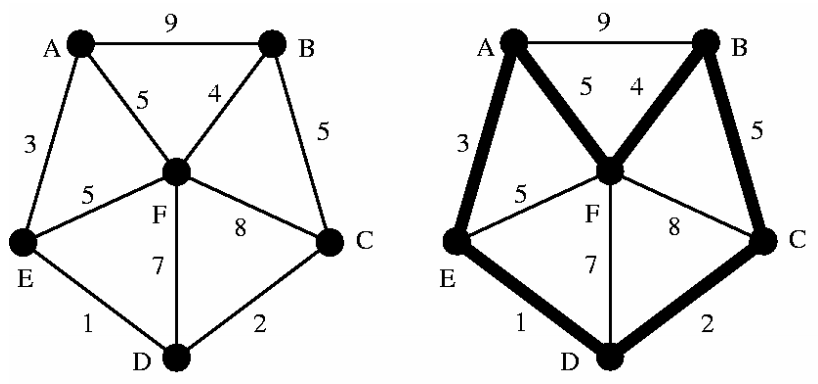
\includegraphics[scale=0.5]{TSP_example.PNG}
\caption{Ví dụ TSP}
\end{figure}

TSP là bài toán NP-hard trong lĩnh vực tối ưu hóa tổ hợp.
\subsection{Bài toán cái túi}
Bài toán cái túi: cho một tập các đồ vật, mỗi đồ vật có hai thông số về khối lượng và giá trị. Đầu ra của bài toán là một tập con đồ vật sao cho tổng trọng lượng của tập nhỏ hơn hoặc bằng một giới hạn cho trước và tổng giá trị của tập đạt giá trị lớn nhất.
\begin{figure}[H]
\center
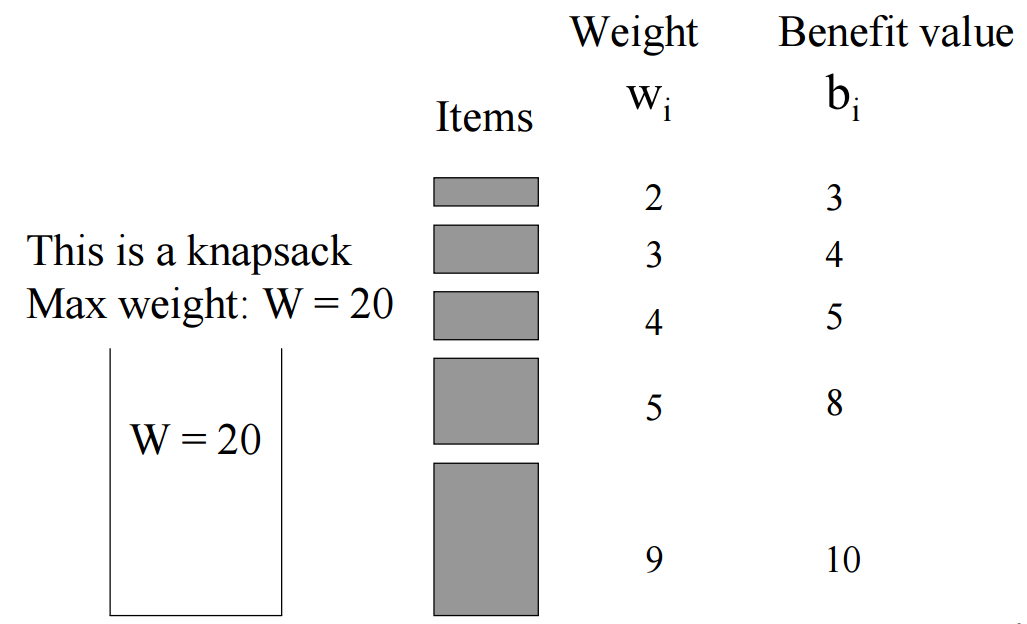
\includegraphics[scale=0.5]{KP_example.PNG}
\caption{Ví dụ cái túi}
\end{figure}

\section{Kết quả thực tế}
\textbf{Bộ tham số}
\begin{itemize}
\item Số lượng cá thể trong quần thể : 50
\item Mức độ đột biến :0.1
\item Tốc độ hội tụ :50
\end{itemize}

\textbf{Kiểu đột biến} : Đột biến một điểm cắt

\subsection{TSP-KP}
\subsection{TSP-KP Kết hợp tích chập}



\begin{thebibliography}{9}
\bibitem{TSP} http://ccf.ee.ntu.edu.tw/~cchen/course/simulation/CAD/unit1A.pdf
\end{thebibliography}
\end{document}
